\documentclass{beamer}
\usepackage[utf8]{inputenc}
\usepackage[english]{babel}
\usepackage[T1]{fontenc}
\usepackage{slide_helper}
\usepackage[inline]{asymptote}
\usepackage{asy_helper}
\usepackage[super]{nth}
\usepackage{array}
\usepackage{wasysym}
\usepackage{pgfplots}
\pgfplotsset{compat=1.5} 
\usepgfplotslibrary{statistics}

\DeclareSymbolFont{extraup}{U}{zavm}{m}{n}
\DeclareMathSymbol{\varheart}{\mathalpha}{extraup}{86}
\DeclareMathSymbol{\vardiamond}{\mathalpha}{extraup}{87}
\DeclareMathSymbol{\varclub}{\mathalpha}{extraup}{84} 
\DeclareMathSymbol{\varspade}{\mathalpha}{extraup}{85}

\newcommand{\suitheart}[1][]{{\color{red}\text{#1}\varheart}}
\newcommand{\suitspade}[1][]{{\color{black}\text{#1}\spadesuit}}
\newcommand{\suitdiamond}[1][]{{\color{red}\text{#1}\vardiamond}}
\newcommand{\suitclub}[1][]{{\color{black}\text{#1}\varclub}}

\newcommand{\prob}[1]{P\left(#1\right)}
\newcommand{\condprob}[2]{\prob{#1~\middle|~#2}}
\newcommand{\comb}[2]{{_{#1}C_{#2}}}
\newcommand{\perm}[2]{_{#1}P_{#2}}

\newcommand{\nullhypothesis}[1]{H_0&:~{#1}}
\newcommand{\althypothesis}[1]{H_A&:~{#1}}


\begin{asydef}
real nd_func(real mu, real sigma, real x) { return 1/sqrt(2*pi*sigma*sigma)*exp((-1*(x-mu)*(x-mu))/(2*sigma*sigma)); }

guide normal_dist(real mu, real sigma, real xmin, real xmax)
{
	real f(real x) { return nd_func(mu, sigma, x); }
	return graph(f, xmin, xmax);
}

void shade_between(real mu, real sigma, real a, real b, pen p=orange)
{
	real f(real x) { return nd_func(mu, sigma, x); }
	guide g = graph(f, a, b);
	
	filldraw((a,0) -- g -- (b,0) -- cycle, p, black);
}

void multiple_nd_curves_example(real std_dev)
{
	size(300, 190, IgnoreAspect);
    
    draw(normal_dist(0, std_dev, -6,6));
    shade_between(0,std_dev,-std_dev,std_dev);
    draw((0,0)--(0,0.45));
    
    label("$\sigma="+format("%#.2f", std_dev)+"$", (-4.2,0.45), Fill(paleyellow));
    
    xaxis(Bottom(), RightTicks(new real[] {-6,-4,-2,0,2,4,6}));
    yaxis(Left(), LeftTicks(size=nan),ymin = 0, ymax = 0.5);
}
\end{asydef}

\begin{asydef}
pair crit = (150, 33);
real a=-1.25;
real b=1.25;
\end{asydef}

\title[MA205 - Section 10.2]{Regression}

\begin{document}
\begin{frame}
\titlepage
\end{frame}

\begin{frame}
\begin{block}{Recall}
Recall that a linear equation (a straight line) is one that can be written as
\begin{equation*}
y=mx+b
\end{equation*}
where $m$ is the slope (\textquote{rise over run}) and $b$ is the y-intercept.
\end{block}\pause

\begin{definition}
Given a collection of paired sample data, the \textbf{regression line} (or \textbf{line of best fit}) is the straight line that \textquote{best} fits the scatter plot of the data. (We will discuss that \textquote{best} means later.)
\end{definition}
\end{frame}

\begin{frame}
\begin{definition}
The \textbf{regression equation} is 
\begin{equation*}
\hat{y}=b_0+b_1 x
\end{equation*}
 algebraically describes the regression line. The regression equation expresses a relationship between $x$ and $\hat{y}$.
\end{definition}\pause

\begin{definition}
We call $x$ the \textbf{explanatory variable}, \textbf{predictor variable}, or \textbf{independent variable}.
\end{definition}\pause

\begin{definition}
We call $y$ the \textbf{response variable}, or \textbf{dependent variable}.
\end{definition}
\end{frame}

\begin{frame}
\begin{note}
We don't use $y=mx+b$ because the format $y=b_0+b_1 x$ can easily be expanded in include more variables:
\begin{equation*}
y=b_0+b_1 x_1 + b_2 x_2 + b_3 x_3 + \cdots
\end{equation*}
This is used when performing a multiple regression.
\end{note}
\end{frame}

\begin{frame}
\begin{block}{Requirements}
The requirements for performing a regression are:
\begin{enumerate}
\item The sample of paired data is a random sample of quantitative data.\pause
\item Visual examination of the scatterplot shows that the points approximate a straight-line pattern.\pause
\item Outliers can have a strong effect on the regression equation, so remove any outliers if they are known errors.
\end{enumerate}
\end{block}
\end{frame}

\begin{frame}
\begin{block}{Slope}
The slope of the regression line is
\begin{equation*}
b_1=r\cdot\dfrac{s_y}{s_x}
\end{equation*}
where $r$ is the linear correlation coefficient, $s_y$ is the standard deviation of the $y$ values, and $s_x$ is the standard deviation of the $x$ values.
\end{block}\pause

\begin{block}{$y$-intercept}
The $y$-intercept of the regression line is
\begin{equation*}
b_0=\bar{y}-b_1\bar{x}
\end{equation*}
where $\bar{y}$ is the sample mean of $y$ values and $\bar{x}$ is the sample mean of $x$ values.
\end{block}\pause

\begin{note}
Technology will calculate both of these values for you.
\end{note}
\end{frame}

\begin{frame}
\begin{block}{Making Predictions}
When making predictions, keep the following in mind:
\begin{description}
\item[Bad Model:] If the regression equation does not appear to be useful for making predictions, don't use the regression equation.\pause
\begin{itemize}
\item The best predicted value of a variable in this case is simply its sample mean.
\end{itemize}\pause
\item[Good Model:] Use the regression equation for predictions only if the graph of the regression line on the scatterplot confirms that the regression line fits the points reasonably well.\pause
\item[Correlation:] Use the regression equation for predictions only if the linear correlation coefficient $r$ indicates that there is a linear correction between the two variables.\pause
\item[Scope:] Use the regression line for predictions only if the data do no go much beyond the scope of available sample data.\pause
\begin{itemize}
\item Predicting too far beyond the scope of the available sample data is called \textbf{extrapolation} and can easily result in bad predictions.
\end{itemize}
\end{description}
\end{block}
\end{frame}

\begin{frame}
\begin{example}
Using the Data Set 16, we can compare a countries chocolate consumption to the number of Nobel laureates.\pause

\vspace{2mm} Technology give a regression line of $\hat{y}=-3.37+2.49x$ and the scatterplot:
\begin{center}
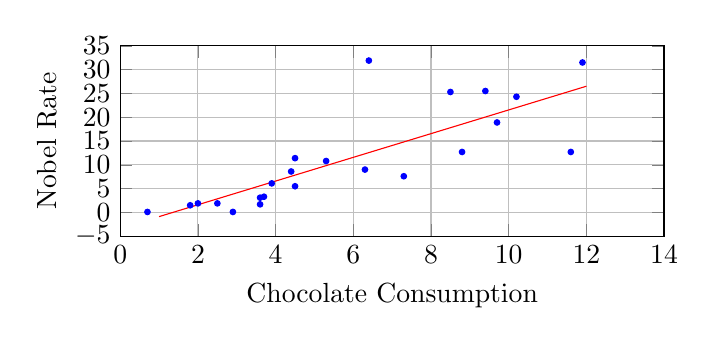
\begin{tikzpicture}
\pgfkeys{/pgf/number format/.cd,
fixed,
precision=999,
set thousands separator={},
1000 sep in fractionals=false,
}
\begin{axis}[
width=0.7\linewidth,
height=4cm,
xlabel={Chocolate Consumption},
ylabel={Nobel Rate},
ymajorgrids=true,
xmajorgrids=true,
%enlarge x limits=false,
%enlarge y limits=false,
xticklabel style={/pgf/number format/.cd,fixed,precision=1},
xticklabel=\pgfmathprintnumber{\tick},
xtick={0,2,...,14},
ytick={-5,0,...,35},
ymin=-5,
ymax=35,
xmin=0,
xmax=14,
scatter/use mapped color={
 %draw=mapped color,
 fill=blue,
},
]
\addplot[scatter, only marks, blue, scatter src=y, mark size=1pt]
coordinates
{
(4.5,5.5)
(10.2,24.3)
(4.4,8.6)
(2.9,0.1)
(3.9,6.1)
(0.7,0.1)
(8.5,25.3)
(7.3,7.6)
(6.3,9)
(11.6,12.7)
(2.5,1.9)
(8.8,12.7)
(3.7,3.3)
(1.8,1.5)
(4.5,11.4)
(9.4,25.5)
(3.6,3.1)
(2,1.9)
(3.6,1.7)
(6.4,31.9)
(11.9,31.5)
(9.7,18.9)
(5.3,10.8)
};
\addplot[domain=1:12, color=red,]{-3.37+2.49*x};
\end{axis}
\end{tikzpicture}
\end{center}\pause
This is a good model, so we can approximate the Nobel Laureate rate for a country that consumes 10kg per capita:

\vspace{-3mm}
\begin{equation*}
\hat{y}=-3.37+2.49(10)\pause =21.5
\end{equation*}\pause

\vspace{-6mm}
So, we expect 21.5 Nobel Laureates per 10 million people.
\end{example}
\end{frame}

\begin{frame}
\begin{example}
The scatterplot shows sample data recording subject height and IQ score.
\begin{center}
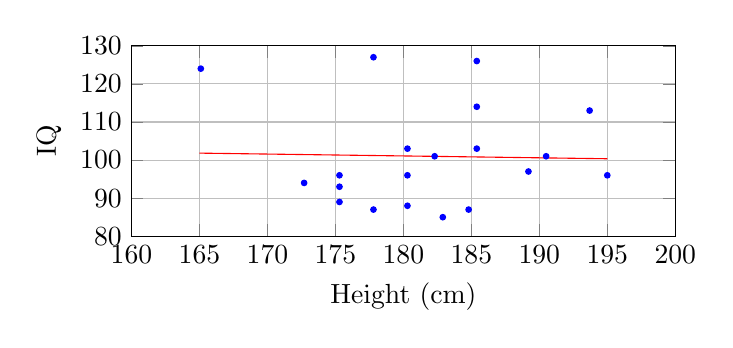
\begin{tikzpicture}
\pgfkeys{/pgf/number format/.cd,
fixed,
precision=999,
set thousands separator={},
1000 sep in fractionals=false,
}
\begin{axis}[
width=0.7\linewidth,
height=4cm,
xlabel={Height (cm)},
ylabel={IQ},
ymajorgrids=true,
xmajorgrids=true,
%enlarge x limits=false,
%enlarge y limits=false,
xticklabel style={/pgf/number format/.cd,fixed,precision=1},
xticklabel=\pgfmathprintnumber{\tick},
xtick={160,165,...,200},
ytick={80,90,...,130},
ymin=80,
ymax=130,
xmin=160,
xmax=200,
scatter/use mapped color={
 %draw=mapped color,
 fill=blue,
},
]
\addplot[scatter, only marks, blue, scatter src=y, mark size=1pt]
coordinates
{
(180.3,96)
(175.3,89)
(184.8,87)
(177.8,87)
(182.3,101)
(185.4,103)
(180.3,103)
(175.3,96)
(177.8,127)
(185.4,126)
(190.5,101)
(195,96)
(175.3,93)
(180.3,88)
(172.7,94)
(182.9,85)
(189.2,97)
(185.4,114)
(193.7,113)
(165.1,124)
};
\addplot[domain=165:195, color=red,]{109.93802-0.04918*x};
\end{axis}
\end{tikzpicture}
\end{center}\pause
The correlation is $r=-0.02731$ and has $P$-value $0.909$. \pause

\vspace{2mm}
This means the regression line is a bad model and should not be used to make predictions.
\end{example}
\end{frame}
\end{document}